%%%%%%%%%%%%%%%%%%%%% chapter.tex 
%%%%%%%%%%%%%%%%%%%%%%%%%%%%%%%%%
%
% sample chapter
%
% Use this file as a template for your own input.
%
%%%%%%%%%%%%%%%%%%%%%%%% Springer-Verlag %%%%%%%%%%%%%%%%%%%%%%%%%%
%\motto{Use the template \emph{chapter.tex} to style the various elements of your chapter content.}

%\chapter{Chapter 0 Security Framework]{Active Directory Tier 0 Security Framework: Cyberattack Prevention and Protection Against Advanced Threats}
%}
\label{intro} % Always give a unique label
% use \chaptermark{}
% to alter or adjust the chapter heading in the running head


\chapter{Reconnaissance}
\begin{abstract}
    abstract text
\end{abstract}
\section{1. Reconnaissance}
Before we jump into exploiting Active Directory, we first need to know what we are working with. Think of reconnaissance as scouting the battlefield before planning an attack. If you do not understand the size of the network you want to attack, how many systems are connected, and what services they might be running, you will, for all intents and purposes, be battling this with your hands tied behind my back, essentially blinded once you try to move forward.

Your main goals here are to map the environment, identify live systems and pay special attention to the machines that stand out as critical-especially Domain Controllers and DNS servers.

\subsection{Defining Reconnaissance}
Reconnaissance is the foundational pre-attack stage of any offensive operation against an Active Directory (AD) environment. At this stage, the attacker's main objective is to gather as much intelligence, data, and information as possible to begin forming a dossier against a victim entity which, in turn, paves the way for shaping the rest of the attack chain. Effective reconnaissance provides you a logical attack map of your target environment, reveals potential weak points, and informs decisions on which systems or targeted users to target first. In Active Directory, reconnaissance often reveals the size of the environment, the role of different systems, and the relationships between domain-joined machines, trusts, relationships, and inter-connected forests.

From a defensive standpoint, this stage is equally important to monitor because reconnaissance often generates anomalous network traffic, host enumeration attempts, and abnormal service scanning activities. Detecting reconnaissance efforts early may prevent an attacker from doing all sorts of malicious activities against your domain and network such as escalating further into the kill chain.

\section{Understanding Your Environment}
Before targeting the environment, you must first understand your own position within the target network. This involves identifying system IP addresses, network subnets, and routing information. In Linux, native commands provide you with quick situational awareness.

\subsection{Know Your \#SHELL}
Identify your IP stack to include IP address and network subnet using native *nix commands such as:

```
\texttt{\# ifconfig}
and
\texttt{\# route -n}
```
\begin{figure}
    \centering
    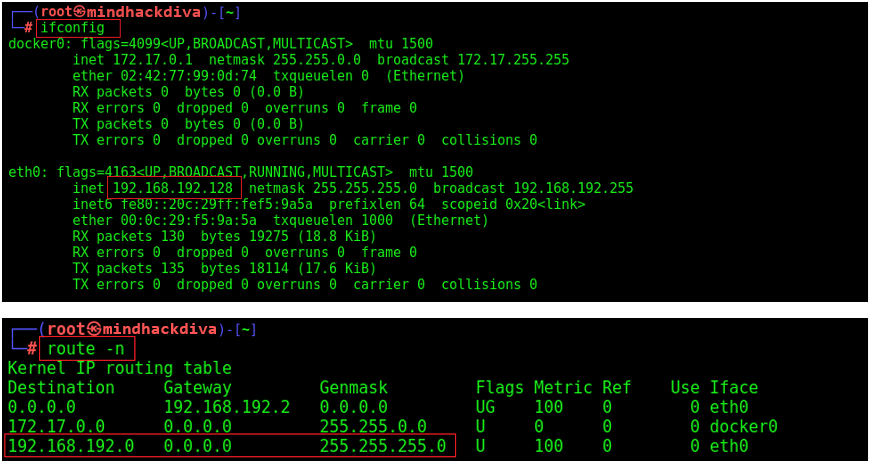
\includegraphics[width=0.75\linewidth]{nixcommands.png}
    \caption{Enter Caption}
\end{figure}
\begin{itemize}
    \item \textbf \texttt{ifconfig} displays your assigned IP address, subnet mask, and interface details. This information ensures you know which segment of the network you are on.
    \item \textbf \texttt{route -n} reveals the routing table, helping you to determine the default gateway, possible VLAN segmentation, and whether your system can reach other subnets.
\end{itemize}

For defenders, unusual use of \texttt{ifconfig} or repeated attempts to probe multiple routes from a non-administrative machine may indicate a compromised host being used as a staging ground.

\subsection{Identifying Potential Targets}
Once network presence has been established, the next step is to identify live hosts and map the subnet(s). This will provide you a list of potential targets for deeper and more concentrated enumeration.
    \label{fig:placeholder}

Host Discovery
Tools such as \texttt{nbtscan} can enumerate NetBIOS names, IP addresses, and associated hostnames within a given subnet, as such:

\begin{verbatim}
# nbtscan -r 192.168.192.0/24

\begin{figure}
    \centering
    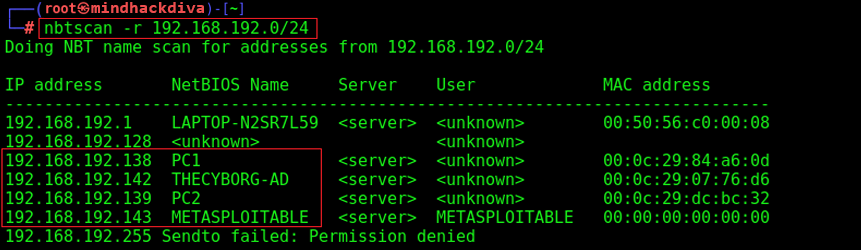
\includegraphics[width=0.75\linewidth]{nbtscan2.png}
    \caption{Enter Caption}
    \label{fig:placeholder}
\end{figure}
\end{verbatim}
This quickly identifies domain-joined machines, file servers, and workstations by resolving their NetBIOS information. Attackers are known to frequently target these assets because hostnames often follow specific naming conventions (e.g., \texttt{DC01}, {FSRV01}, {HR-LAPTOP23} that reveal system roles or ownership.

\textbf{Defensive Note:}
Unusual NetBIOS scanning across an entire subnet is an early Indicator of Compromise (IOC). Defenders and security teams can monitor for excessive \texttt{nbtscan}-like traffic or NetBIOS broadcast floods.

\subsubsection{Service and Port Scanning}
After you have identified some live hosts, you must now determine what services they may be exposing. This is where Nmap becomes a critical tool, and one of your best friends. Take the below Nmap command, for example:
\begin{verbatim}
# nmap -sS -p- -T4 192.168.192.10
```
\begin{figure}
    \centering
    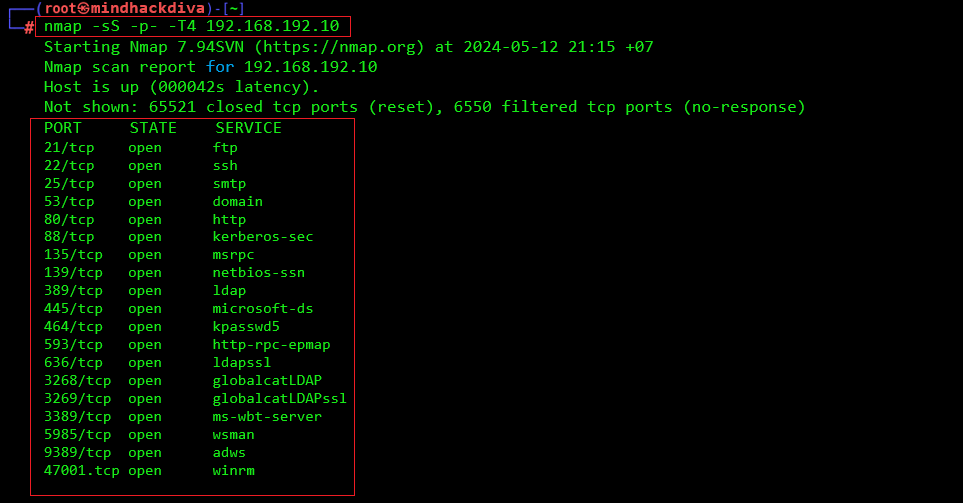
\includegraphics[width=0.75\linewidth]{nmapfulltcp.png}
    \caption{Enter Caption}
\end{figure}
\end{verbatim}

This Nmap command launches a full TCP SYN (\texttt{-sS} ) across all 65,536 ports (\texttt{-p-}), with a timing template of 4 (\texttt{-T4}), aggressive but not insane speed).
\begin{itemize}
    \item \textbf \texttt{-sS:} Conducts a stealth SYN scan (half-open scan).
    \item \textbf \texttt{-p-:} Enumerates all 65,536 TCP ports, ensuring no service is skipped or missed.
    \item \textbf \texttt{-T4:} Balances speed with stealth, faster than default but less noisy than \texttt{-T5}.
\end{itemize}

For Active Directory attacks, particular focus should be given to the Domain Controllers, as they are the backbone of identity and access management. Commonly targeted network ports include, but are not limited to:
\begin{itemize}
    \item \textbf{53 (DNS):} Domain name resolution.
    \item \textbf{88 (Kerberos):} Authentication services; vital for Kerberoasting and ticket abuse.
    \item \textbf{135 (RPC):} Remote Procedure Calls; often abused for enumeration.
    \item \textbf{389 (LDAP):} Directory queries; rich in user and group information.
    \item \textbf{445 (SMB):} File sharing, lateral movement, and Pass-the-Hash (PtH) exploitation.
    \item \textbf{464 (Kerberos password change):} Abuse potential for password spraying attacks.
    \item \textbf{636 (LDAPS):} Secure LDAP queries.
    \item \textbf{3268 / 3269 (Global Catalog):} Queries across multi-domain forests.
\end{itemize}

\subsubsection{Scanning the Domain Controller Scenario}
Suppose during reconnaissance, you identify a potential Domain Controller (DC) at IP address \texttt{192.168.192.10.} A targeted Nmap scan against well-known Active Directory-related ports can quickly reveal the key services it is running. For example, the following command performs a focused version scan:
\texttt{\# nmap -sV -p 53,88,135,389,445,464,636,3268,3269 192.168.192.10}

Let us break this command down so that you have a firm grasp as to what the command is actually performing for you:
\texttt{-sV (Service Detection):} This switch tells Nmap to probe each open port to determine the exact service and software version. Instead of simply knowing that port 389 is "LDAP," you can often learn whether it is \textit{Microsoft Active Directory LDAP} on a specific Windows Server build, or even a vendor's custom LDAP implementation. This level of detail is critical for attackers seeking vulnerable versions and equally valuable for defenders validating patch levels.
\texttt{-p 53,88,135,389.445.464.636.3268.3269 (Port Specification):} Instead of scanning all 65,535 ports, this Nmap command narrows the scope to Active Directory's most important services, reducing noise and scan duration. The chosen ports directly map to ADs core functionality:
53/tcp (DNS): AD-integrated DNS, fundamental for domain-wide name resolution and locating domain controllers.
88/tcp (Kerberos): Kerberos authentication traffic; critical for tickets (TGT / TGS) and often targeted by Kerberoasting.
135/tcp (MS RPC): Microsoft Remote Procedure Call endpoint mapper; a common vector for enumeration and lateral movement.
389/tcp (LDAP): Lightweight Directory Access Protocol; used for directory queries. Misconfigurations here often expose sensitive information.
445/tcp (SMB): Server Message Block; vital for file shares and authentication relay. Older versions (SMBv1) are extremely vulnerable.
464/tcp (Kerberos Change / Set Password): Used for password changes within Kerberos authentication.
636/tcp (LDAPS): LDAP over SSL/TLS; often targeted if improperly configured with weak encryption.
3268/tcp (Global Catalog LDAP): Provides forest-wide LDAP queries; useful for enumerating objects across domains.
3269/tcp (Global Catalog LDAP over SSL): Secure version of the Global Catalog query service.

If you specifically focus on these ports,you can greatly accelerate your recon efforts by saving time, and minimizing network traffic "noise" that might otherwise be flagged by defensive monitoring systems.
 Furthermore, the output of this scan will usually reveal service banners and version details. For instance, you might learn that SMB is running Microsoft Windows 7 SMBv1 (and yes, they are out there), immediately signaling the possibility of an \textit{EternalBlue-style exploit.} Or LDAP may expose that the server is running a legacy schema that has not been hardened. This type of reconnaissance forms your foundation for determining attack pathways (for red teamers) or hardening priorities (for blue teamers).



The output typically reveals critical services and their versions, enabling you to determine potential vulnerabilities such as outdated SMB versions or misconfigured LDAP services.

\textbf{Defensive Note:}
Defenders and security teams can baseline expected port scans in their environment. A sudden surge of connections across multiple AD-specific ports may indicate adversarial reconnaissance. Employing honeypots or canary services on non-production IPs can catch this early.

\subsection{Reconnaissance Goals Recap}
By the conclusion of reconnaissance, you should have:
\begin{itemize}
    \item A comprehensive understanding of your target environment, to include:
    \begin{itemize}
        \item Detailed information about the target network architecture and topology information, to include:
        \begin{itemize}
            \item IP addresses, subnet masks, and network ranges
            \item Identification of active systems and services: including their versions and the potential vulnerabilities they may carry
            \item Knowledge of potential entry points and attack pathways: such as open ports and weak security configurations
            \item Information on security policies and deployed security tools: such as firewalls or intrusion detection systems
            \item Details about potential third-party connections or vulnerabilities
            \item Potentially, information on key personnel to aid in social engineering tactics
        \end{itemize}
    \end{itemize}
\end{itemize}

In essence, your goal for reconnaissance is to gather as much information you can on your target or opponent to provide a comprehensive picture of the target's security stance. This information can then be used to further plan and execute more targeted and effective attacks (or, for defenders, to strengthen defenses and mitigate risks in an expedient and efficient manner).